\documentclass{article}
\usepackage{amsmath, amssymb}
\usepackage{amsmath}
\usepackage[active]{srcltx}
\usepackage{amssymb}
\usepackage{amscd}
\usepackage{makeidx}
\usepackage{amsthm}
\usepackage{algpseudocode}
\usepackage{graphicx}
\usepackage{algorithm}
\usepackage[utf8]{inputenc}
\renewcommand{\baselinestretch}{1}
\setcounter{page}{1}
\setlength{\textheight}{21.6cm}
\setlength{\textwidth}{14cm}
\setlength{\oddsidemargin}{1cm}
\setlength{\evensidemargin}{1cm}
\pagestyle{myheadings}
\thispagestyle{empty}
\date{}
\begin{document}
\centerline{\bf Neural Networks, Sem: 2019-1, 3CM1, Primer entrega de proyecto, 2016630234, 12-11-2018}
\centerline{}
\centerline{}
\begin{center}
\Large{\textsc{Primer entrega: Reporte Perceptron multicapa}}
\end{center}
\centerline{}
\centerline{\bf {Equipo 4}}
\centerline{Amezcua Arevalo Bruno}
\centerline{Mart\'inez Cer\'on Jos\'e Emmanuel}
\centerline{G\'omez Reus Jorge}
\centerline{}
\centerline{Escuela Superior de C\'omputo}
\centerline{Instituto Polit\'ecnico Nacional, M\'exico}
\centerline{$Marco Antonio Moreno Armendariz$}
\newtheorem{Theorem}{\quad Theorem}[section]
\newtheorem{Definition}[Theorem]{\quad Definition}
\newtheorem{Corollary}[Theorem]{\quad Corollary}
\newtheorem{Lemma}[Theorem]{\quad Lemma}
\newtheorem{Example}[Theorem]{\quad Example}
\bigskip

\section{Introducci\'on}

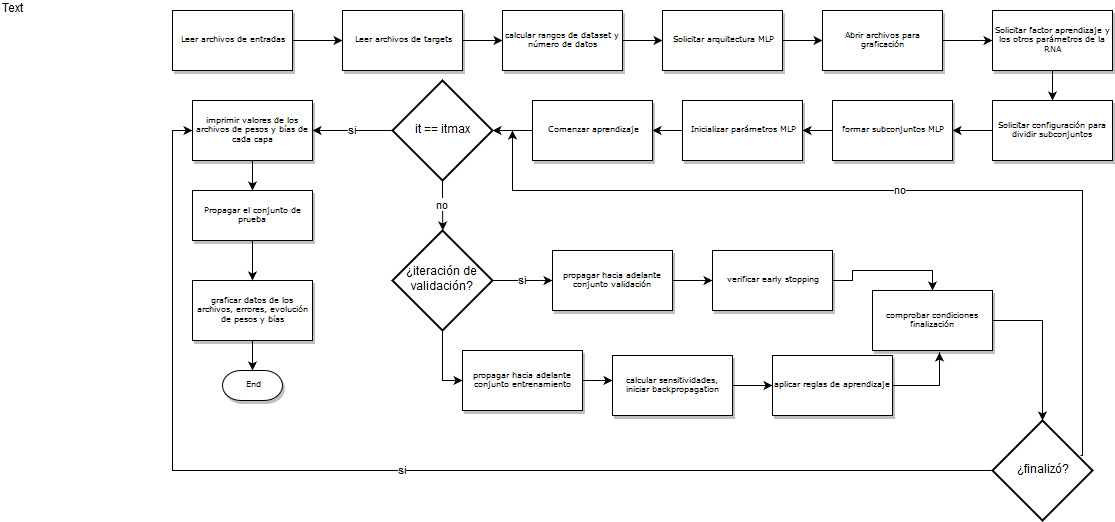
\includegraphics[scale=0.5]{2.jpeg}

\subsection{Seudoc\'odigo}
\textbf{Descripción del algoritmo}

 \begin{algorithm}
\caption{MLP Entrenamiento}\label{euclid}
\begin{algorithmic}[1]
\Procedure{Leer archivo de entradas}{}
\EndProcedure
\State
\Procedure{Leer archivo targets}{}
\EndProcedure
\State
\Procedure{Calcular rangos y bumero de datos}{}
\EndProcedure
\State
\State arq = input(Ingresar la arquitectura del MLP:)
\State fns = input (Ingresar las funciones de activaci\'on)
\State Abrir los archivos para gratificaci\'on
\State
\For{(i$=$1; i$<$ NumeroDeCapas; i++)} 
	\State archivos\_pesos $+=$ 1
	\State archivos\_bias += 1
	\State crear/abrir archivo pesos
	\State crear/abrir archivo bias
\EndFor
\Procedure{Solicidar parametros de la RNA}{valor del factor de aprendizaje, error de \'epoca, itmax, etc}
\EndProcedure
\State
\Procedure{Solicitar configuracion para dividir subconjuntos}{80-10-10, 70-15-15}
\EndProcedure
\State
\Procedure{Formar subconjuntos}{}
\EndProcedure
\State
\Procedure{Inicializar matriz de pesos y el vector bias con valaores aleatorios entre -1 y 1}{}
\EndProcedure
\State
\State W = cell(n\'umero de capas, 1)
\State b = cell(n\'umero de capas, 1)
\State \%\% Salidas de la capa
\State a = cell(n\'umero de capas, 1)
\State \%\% Sensitividades
\State S = cell (n\'umero de capa, 1)
\State F\_m = cell(n\'umero de capas, 1)

\For{(j=1; i$<=$numeroDeCapas; i++)}
    \State W{i} = rand() \% (1) -1;
    \State b{i} = rand() \% (1) -1;
    \State guardar archivo
\EndFor
\end{algorithmic}
\end{algorithm}


 \begin{algorithm}
\caption{MLP Aprendizaje}\label{euclid}
\begin{algorithmic}[2]
\State early\_stopping = false
\State error\_val = 0
\State error\_apr = 0
\State num\_itval = 0
\For{(it\_max)}
\State Verificar error en validaci\'on
\If{(it \% itval != 0)}
    \For{(Datos de Entrenamiento)}
        \Procedure{Propagar datos de entrenamiento}{}
        \EndProcedure
    \EndFor
    \State
    \For{(N\'umero de capas)}
        \Procedure{Propagar cada dato}{}
        \EndProcedure
        \Procedure{Calcular errores}{}
        \EndProcedure
        \State
        \Procedure{Calcular Sensitividades}{}
        \EndProcedure
        \State
        \Procedure{Backpropagation}{}
        \EndProcedure
        \State
        \Procedure{Obtener funci\'on de activaci\'on para la capa}{}
        \EndProcedure
        \State
        \Procedure{Aplicar reglas de aprendizaje}{}
        \EndProcedure
        \State
    \EndFor
    \Procedure{Calcular el error de aprendizaje y guardarlo}{}
    \EndProcedure
    \State
    \Else
        \For{(datos validaci\'on)}
            \Procedure{Propagar hacia adelante los elementos del conjunto de validaci\'on}{}
            \EndProcedure
            \State
            \For{(N\'umero de capas)}
                \Procedure{Propagar cada dato}{}
                \EndProcedure
            \EndFor
        \Procedure{Calcular error de validaci\'on}{}
        \EndProcedure
        \EndFor
    \Procedure{Verificar errores para early stopping}{}
    \EndProcedure
\EndIf
\Procedure{Comprobar condiciones de finalizaci\'on}{}
\EndProcedure
\EndFor
\end{algorithmic}
\end{algorithm}

 \begin{algorithm}
\caption{MLP Prueba}\label{euclid}
\begin{algorithmic}[3]
\If{(early\_stopping == true)}
    \Procedure{Imprimir en un archivo los \'ultimos valores de pesos y bias de cada capa}{}
    \EndProcedure
    \State
    \For(N\'umero de capas)
        \State Imprimir dato de pesos
        \State Imprimir dato de bias
    \EndFor
\EndIf

\Procedure{Propagar conjunto de prueba}{}
\EndProcedure
        \State
\For{(N\'umero de elementos de prueba)}
    \For{(N\'umero de capas)}
        \Procedure{Propagar cada dato}{}
        \EndProcedure
    \EndFor
\EndFor
\Procedure{Graficar el conjunto de prueba y targets contra resultados de la red}{}
\EndProcedure
\end{algorithmic}
\end{algorithm}
\end{document}
